\documentclass[11pt,a4paper]{article}
\usepackage[margin=2.3cm]{geometry}
\IfFileExists{lmodern.sty}{\usepackage[T1]{fontenc}\usepackage{lmodern}\usepackage{microtype}}{}
\usepackage{amsmath,amssymb}
\usepackage{graphicx,booktabs,float,caption,subcaption}
\usepackage{algorithm,algpseudocode}
\usepackage[hidelinks]{hyperref}
\captionsetup{font=small}

\title{Clustering and Initialization:\\ k-means versus k-means++\\[4pt]
\large Statistical Methods for Machine Learning --- Experimental Project, A.Y.\ 2025/26}
\author{Aliza Aziz \\ Student ID: \texttt{82838A} \\ Università degli Studi di Milano}
\date{\today}

\begin{document}
\maketitle

\begin{abstract}
We study how the initialization of Lloyd's algorithm affects the quality and the
variability of k-means clustering. We implement from scratch, in Python and numpy,
the classical random initialization and the $D^2$ seeding of k-means++
(Arthur and Vassilvitskii, SODA 2007), and compare them over many paired random
trials on a synthetic dataset that replicates the one used in the paper, on a 2-D
toy dataset, and on a real high-dimensional multiclass dataset (UCI handwritten
digits). On well-separated synthetic clusters, random seeding gets trapped in
local minima whose cost is thousands of times the best one, while k-means++ finds
the best solution in every run and converges in a single iteration. On the real
dataset the advantage is small but consistent. Two extensions show that the gap
grows with cluster separation and is essentially independent of dimension.
\end{abstract}

\section{Introduction and problem setting}

Given points $\mathcal{X}=\{x_1,\dots,x_n\}\subset\mathbb{R}^d$ and an integer $k$,
k-means looks for $k$ centres $C=\{c_1,\dots,c_k\}$ minimizing the
\emph{inertia} (also called potential, or within-cluster sum of squares)
\begin{equation}\label{eq:phi}
\phi(C)=\sum_{i=1}^n \min_{c\in C}\lVert x_i-c\rVert^2 .
\end{equation}
In the language of the course this is empirical risk minimization with the
squared loss over the class of ``nearest-centre'' quantizers. The problem is
NP-hard and the objective is non-convex, so in practice it is attacked with
\emph{Lloyd's algorithm}: starting from some centres, repeat (i) assign every
point to its closest centre, (ii) move every centre to the mean of its points.
Both steps can only decrease $\phi$, so the algorithm terminates, but only at a
\emph{local} minimum, and which one depends entirely on the starting centres.
Two runs on the same data may therefore end in very different solutions.

Arthur and Vassilvitskii proposed k-means++, a randomized seeding rule ($D^2$
sampling) that picks well spread-out centres, and proved that the seeding
\emph{alone} already satisfies
\begin{equation}\label{eq:bound}
\mathbb{E}[\phi(C_{\text{seed}})]\le 8(\ln k+2)\,\phi_{\mathrm{OPT}},
\end{equation}
while uniform random seeding has no such guarantee. Lloyd iterations can only
improve on this. The goal of this project is to measure empirically how much this
matters: (a) the distribution of final inertia over many runs, (b) its
variability, and (c) the stability of the obtained partitions.

\section{Algorithms and implementation}

All code is in \texttt{src/kmeans.py}. Only numpy is used, to vectorize
arithmetic and to sample random numbers; no clustering routine from any library
is called. scikit-learn is used only to \emph{load} the digits dataset and, in
\texttt{tests/}, as an independent reference to check our Adjusted Rand Index.

\paragraph{Random initialization.} $k$ distinct data points are drawn uniformly
without replacement (the usual ``Forgy'' scheme, also the baseline of the paper).

\paragraph{k-means++ ($D^2$ seeding).} Let $D(x)$ be the distance of $x$ to the
closest centre already chosen.
\begin{algorithm}[H]
\caption{$D^2$ seeding (k-means++)}
\begin{algorithmic}[1]
\State $c_1 \gets$ a data point chosen uniformly at random
\For{$i=2,\dots,k$}
  \State compute $D(x)^2$ for every $x\in\mathcal X$
  \State $c_i \gets x$ with probability $D(x)^2/\sum_{y\in\mathcal X} D(y)^2$
\EndFor
\State \Return $\{c_1,\dots,c_k\}$
\end{algorithmic}
\end{algorithm}
\noindent Points far from all current centres are much more likely to be chosen, so
the centres spread over the data, but the rule is still random, which protects it
from single outliers (a deterministic ``farthest point'' rule would always pick
them). We keep a vector of the current $D(x)^2$ and update it with one distance
computation per new centre, so seeding costs $O(nkd)$, the same as one Lloyd
iteration.

\paragraph{Lloyd's algorithm.} Shared by both methods, so any difference in the
results is due to the seeding alone. Squared distances are computed in matrix
form as $\lVert x\rVert^2-2x^\top c+\lVert c\rVert^2$. Iterations stop when the
assignment no longer changes (an exact fixed point), with a safety cap of 300
iterations that was never reached. If a cluster becomes empty, its centre is moved
to the point that is currently worst served; this keeps exactly $k$ clusters and
never increases $\phi$. The same rule applies to both methods.

\paragraph{Correctness checks.} \texttt{tests/test\_kmeans.py} verifies that the
fast distance formula matches a brute-force computation, that the objective never
increases along Lloyd iterations, that $D^2$ seeding returns distinct points, that
three obviously separated clusters are recovered exactly, and that our Adjusted
Rand Index equals scikit-learn's on random labelings.

\section{Datasets}

The assignment requires a synthetic dataset with good clustering potential and a
real-world high-dimensional multiclass dataset; we use both, plus a 2-D toy set
for visualization and two synthetic families for the extensions.

\begin{itemize}
\item \textbf{Norm-25 (synthetic).} The synthetic set of the paper: 25 ``true''
centres drawn uniformly in $[0,500]^{15}$, and 200 points per centre drawn from an
isotropic Gaussian with unit variance ($n=5000$, $d=15$). The clusters are tiny
compared with their distances, so the true partition is (with overwhelming
probability) the optimal one for $k=25$ and is known. This is the setting where
initialization should matter the most, and the one where the paper reports the
largest gains.
\item \textbf{Blobs-2D (synthetic).} Nine Gaussian clusters ($\sigma=0.6$) on a
$3\times3$ grid with spacing 5, 150 points each. Used to \emph{see} local minima.
\item \textbf{UCI Digits (real).} The UCI ``Optical Recognition of Handwritten
Digits'' data: 1797 images of $8\times8$ pixels, $d=64$, 10 classes. It is an
MNIST-like dataset (as suggested in the assignment), but small enough to run
hundreds of clusterings in seconds, and it ships with scikit-learn so the project
runs offline. All features are pixel intensities on the same scale $0$--$16$, so
we do not standardize them: rescaling would change the geometry k-means relies on.
\item \textbf{Extensions.} (i) \emph{Overlap:} 10 centres in $[0,10]^{10}$ with
cluster spread $\sigma\in\{0.25,0.5,1,2,4\}$, from clearly separated to strongly
overlapping. (ii) \emph{Dimension:} the Norm-25 generator with 100 points per
cluster and $d\in\{2,5,15,50,100\}$.
\end{itemize}

\paragraph{Evaluation protocol and data leakage.} Clustering is unsupervised and
the object of study is the \emph{optimization} of $\phi$ on a given dataset, so,
as in the paper, each algorithm is run and evaluated on the same set of points;
there is no prediction on unseen data to evaluate, hence no train/test split for
the main experiments. The true labels are never given to the algorithms; they are
used only afterwards to compute the agreement with the ground truth. As a sanity
check that the centres are not ``overfitting'' the sample, we also learnt
$k=10$ centres on a random 80\% of Digits and measured the per-point cost on the
remaining 20\% (Section~\ref{sec:real}).

\section{Experimental design and metrics}

For each dataset and each $k$ we run \textbf{50 trials} of each method
(20 trials per point in the extensions). Trial $t$ uses the random seed $t$ for both
methods (a paired design), so every number in this report is reproducible by
running \texttt{python run\_experiments.py}. Following the paper we use
$k\in\{10,25,50\}$ on Norm-25 and on Digits, which includes the ``correct'' value
(25 and 10, respectively) as well as under- and over-clustering. We record:
\begin{itemize}
\item \textbf{seed inertia}: $\phi$ right after seeding, before any Lloyd step;
\item \textbf{final inertia} and the \textbf{ratio} final/best, where ``best'' is the
lowest inertia found by \emph{any} run of either method on that configuration
(a proxy for $\phi_{\mathrm{OPT}}$);
\item \textbf{variability}: standard deviation, coefficient of variation
(CV $=$ std/mean), worst ratio, and \textbf{hit\%}, the fraction of runs within
0.1\% of the best;
\item \textbf{stability of the partition}: the mean Adjusted Rand Index (ARI)
between the partitions produced by every pair of runs (1225 pairs). ARI equals 1
for identical partitions (up to renaming clusters) and is about 0 for random
agreement. This measures stability of the \emph{output}, not just of the cost;
\item \textbf{ARI with the ground truth} when $k$ equals the number of classes;
\item number of Lloyd iterations and wall-clock time.
\end{itemize}

\section{Results}

\subsection{Synthetic data: Norm-25}

\begin{table}[ht]\centering\small
\caption{Results on \texttt{Norm-25} over 50 paired trials per method. Ratio = final inertia divided by the best inertia found by any run; \emph{hit} = runs within 0.1\% of the best; pair ARI = mean agreement between partitions of two runs.}
\label{tab:Norm25}
\resizebox{\textwidth}{!}{\begin{tabular}{llrrrrrrrrrr}\toprule
$k$ & method & seed inertia & final mean & final std & CV\% & ratio mean & ratio max & hit\% & iters & pair ARI & ARI truth\\\midrule
10 & random & $1.327\mathrm{e}9$ & $7.398\mathrm{e}8$ & $5.913\mathrm{e}7$ & 7.99 & 1.224 & 1.436 & 0 & 6.7 & 0.355 & --\\
10 & k-means++ & $1.122\mathrm{e}9$ & $6.790\mathrm{e}8$ & $3.688\mathrm{e}7$ & 5.43 & 1.123 & 1.263 & 2 & 1.5 & 0.421 & --\\
\midrule
25 & random & $5.871\mathrm{e}8$ & $2.375\mathrm{e}8$ & $6.096\mathrm{e}7$ & 25.66 & 3{,}181.805 & 5{,}079.173 & 0 & 15.6 & 0.561 & 0.697\\
25 & k-means++ & $1.492\mathrm{e}5$ & $7.466\mathrm{e}4$ & $0$ & 0.00 & 1.000 & 1.000 & 100 & 1.0 & 1.000 & 1.000\\
\midrule
50 & random & $2.038\mathrm{e}8$ & $3.912\mathrm{e}7$ & $3.768\mathrm{e}7$ & 96.33 & 557.846 & 2{,}036.614 & 0 & 20.0 & 0.586 & --\\
50 & k-means++ & $1.273\mathrm{e}5$ & $7.033\mathrm{e}4$ & $1.224\mathrm{e}2$ & 0.17 & 1.003 & 1.007 & 12 & 18.8 & 0.640 & --\\
\bottomrule\end{tabular}}\end{table}

\begin{table}[ht]\centering\small
\caption{Results on \texttt{Digits} over 50 paired trials per method. Ratio = final inertia divided by the best inertia found by any run; \emph{hit} = runs within 0.1\% of the best; pair ARI = mean agreement between partitions of two runs.}
\label{tab:Digits}
\resizebox{\textwidth}{!}{\begin{tabular}{llrrrrrrrrrr}\toprule
$k$ & method & seed inertia & final mean & final std & CV\% & ratio mean & ratio max & hit\% & iters & pair ARI & ARI truth\\\midrule
10 & random & $2.280\mathrm{e}6$ & $1.188\mathrm{e}6$ & $2.673\mathrm{e}4$ & 2.25 & 1.020 & 1.090 & 24 & 20.1 & 0.753 & 0.618\\
10 & k-means++ & $2.250\mathrm{e}6$ & $1.188\mathrm{e}6$ & $2.580\mathrm{e}4$ & 2.17 & 1.019 & 1.088 & 12 & 19.0 & 0.751 & 0.610\\
\midrule
25 & random & $1.684\mathrm{e}6$ & $9.034\mathrm{e}5$ & $9.664\mathrm{e}3$ & 1.07 & 1.023 & 1.059 & 0 & 22.6 & 0.643 & --\\
25 & k-means++ & $1.626\mathrm{e}6$ & $9.009\mathrm{e}5$ & $1.002\mathrm{e}4$ & 1.11 & 1.020 & 1.057 & 2 & 20.3 & 0.655 & --\\
\midrule
50 & random & $1.319\mathrm{e}6$ & $7.363\mathrm{e}5$ & $9.383\mathrm{e}3$ & 1.27 & 1.030 & 1.062 & 2 & 18.8 & 0.545 & --\\
50 & k-means++ & $1.288\mathrm{e}6$ & $7.319\mathrm{e}5$ & $7.093\mathrm{e}3$ & 0.97 & 1.024 & 1.043 & 0 & 18.4 & 0.562 & --\\
\bottomrule\end{tabular}}\end{table}

\begin{table}[ht]\centering\small
\caption{Results on \texttt{Blobs-2D} over 50 paired trials per method. Ratio = final inertia divided by the best inertia found by any run; \emph{hit} = runs within 0.1\% of the best; pair ARI = mean agreement between partitions of two runs.}
\label{tab:Blobs2D}
\resizebox{\textwidth}{!}{\begin{tabular}{llrrrrrrrrrr}\toprule
$k$ & method & seed inertia & final mean & final std & CV\% & ratio mean & ratio max & hit\% & iters & pair ARI & ARI truth\\\midrule
9 & random & $1.161\mathrm{e}4$ & $2.553\mathrm{e}3$ & $1.232\mathrm{e}3$ & 48.26 & 2.651 & 4.930 & 30 & 9.3 & 0.788 & 0.878\\
9 & k-means++ & $3.509\mathrm{e}3$ & $1.444\mathrm{e}3$ & $8.912\mathrm{e}2$ & 61.71 & 1.500 & 4.815 & 76 & 4.7 & 0.926 & 0.962\\
\bottomrule\end{tabular}}\end{table}


\begin{figure}[ht]\centering
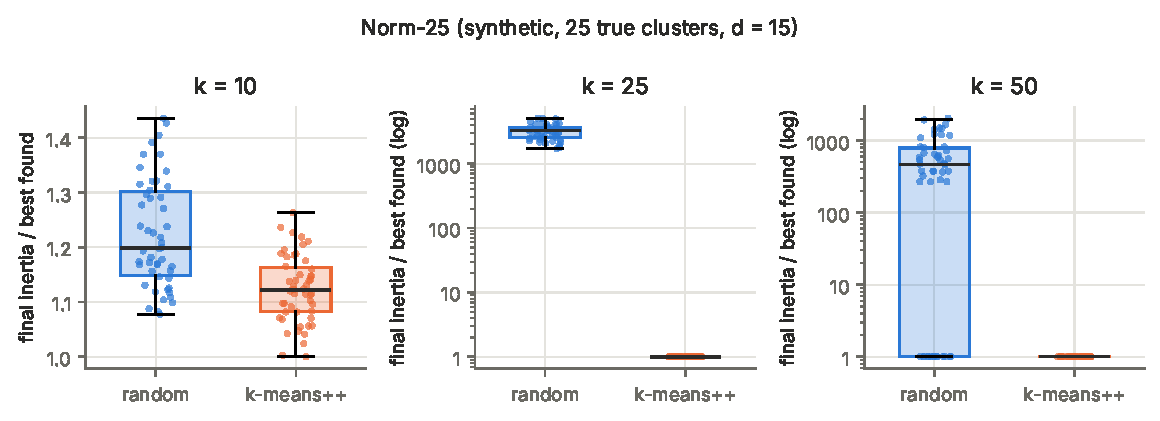
\includegraphics[width=\textwidth]{figures/norm25_box.pdf}
\caption{Norm-25: distribution of final inertia relative to the best found,
50 runs per method (each dot is one run). Note the log scale for $k=25,50$.}
\label{fig:normbox}
\end{figure}

Table~\ref{tab:Norm25} and Figure~\ref{fig:normbox} show the most striking result.
For $k=25$, \textbf{k-means++ reached the best solution in 50 out of 50 runs},
with zero variance, perfect agreement with the true clusters (ARI $=1$) and with
each other (pair ARI $=1$). \textbf{Random seeding never reached it}: its final
inertia is on average about \textbf{3200 times} the best (worst run $\approx5100$
times), with CV 26\%, and its partitions agree with the truth only at ARI
$\approx0.70$.

The reason is geometric. A run of random seeding succeeds only if every one of
the 25 equally sized clusters receives exactly one initial centre, which happens
with probability $25!/25^{25}\approx1.7\times10^{-10}$. Otherwise some true
cluster gets two centres and another gets none, and Lloyd's algorithm cannot
repair this: a centre that sits inside a cluster 500 units away from the empty one
never ``sees'' its points, so two far-apart true clusters end up merged and the
cost explodes (each merged pair contributes a squared distance of order
$500^2\cdot d/6$ per point). With $D^2$ seeding, once a cluster contains a centre
its points have $D(x)^2\approx d\sigma^2=15$, whereas points of uncovered clusters
have $D(x)^2$ in the order of $10^5$--$10^6$; the next centre is thus almost
certainly drawn from an uncovered cluster. This is why k-means++ is
\emph{already} essentially optimal after seeding: its seed inertia is $2.0$ times
the best (each point is measured from a random point of its cluster instead of the
mean, which doubles the expected cost of a Gaussian cluster), well inside the bound
\eqref{eq:bound}, which for $k=25$ is $8(\ln 25+2)\approx 41.8$. One Lloyd
iteration then moves every centre to its cluster mean and the algorithm stops:
\textbf{1.0 iteration on average against 15.6} for random seeding
(Figure~\ref{fig:conv}, left). The seed inertia of random seeding, by contrast, is
about 7900 times the best.

For $k=50$ (more centres than true clusters) random seeding still fails most of
the time (CV 96\%, mean ratio $\approx560$), because the chance of leaving some
cluster empty remains high; a few lucky runs reach a ratio close to 1, which is
why its box spans three orders of magnitude. k-means++ is within $0.7\%$ of the
best in every run. Here the optimum is not unique-looking anymore (the 25 extra
centres can split clusters in many nearly equivalent ways), which explains why
the pair ARI of k-means++ is only $0.64$ even though the cost is almost constant:
\emph{different partitions with the same cost} are a form of instability that the
inertia alone does not reveal. For $k=10$ (fewer centres than clusters) both
methods must merge clusters; k-means++ is still better (mean ratio $1.12$ vs
$1.22$) but neither finds the best grouping reliably.

\begin{figure}[ht]\centering
\begin{subfigure}{0.49\textwidth}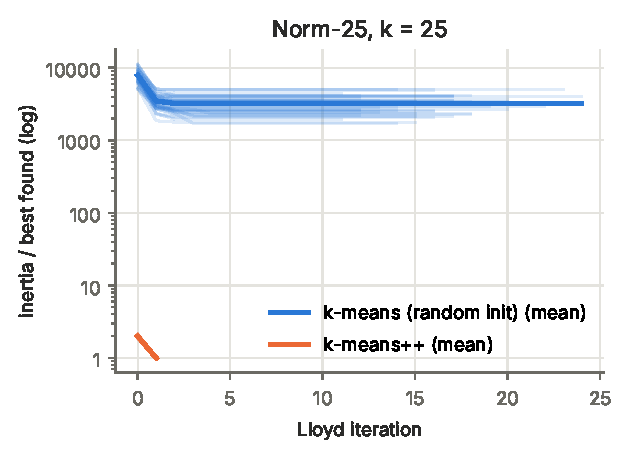
\includegraphics[width=\textwidth]{figures/norm25_convergence.pdf}\end{subfigure}
\begin{subfigure}{0.49\textwidth}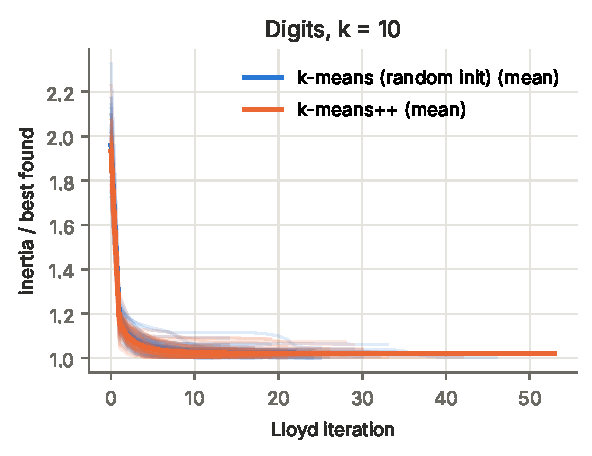
\includegraphics[width=\textwidth]{figures/digits_convergence.pdf}\end{subfigure}
\caption{Inertia (relative to the best) along Lloyd iterations; thin lines are
single runs, thick lines are means. Iteration 0 is the cost of the seeding.}
\label{fig:conv}
\end{figure}

\subsection{Visualizing local minima: Blobs-2D}

Figure~\ref{fig:blobs} shows the worst of 50 runs of each method on the 2-D grid.
In both cases the failure has the same shape: two centres share one blob and a
single centre is left halfway between two blobs. Random seeding reached the best
solution in 30\% of the runs, k-means++ in \textbf{76\%}; mean ratios are 2.65 and
1.50, and the mean ARI with the truth is $0.88$ vs $0.96$. This is an honest
negative aspect: k-means++ is not a guarantee of optimality, only a guarantee in
expectation, and with clusters this close (spacing 5, $\sigma=0.6$) the
$D^2$ distribution still puts some mass on already covered blobs. Its worst run
is about as bad as the worst random run; what changes is how often it happens.

\begin{figure}[ht]\centering
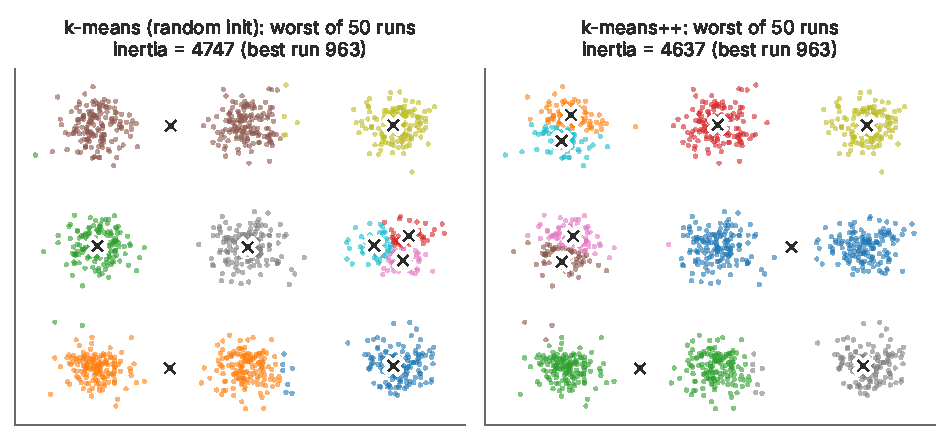
\includegraphics[width=0.9\textwidth]{figures/blobs2d_worst.pdf}
\caption{Blobs-2D, $k=9$: worst run out of 50 for each method. Crosses are the
final centres, colors the final clusters.}
\label{fig:blobs}
\end{figure}

\subsection{Real-world data: UCI Digits}\label{sec:real}

\begin{figure}[ht]\centering
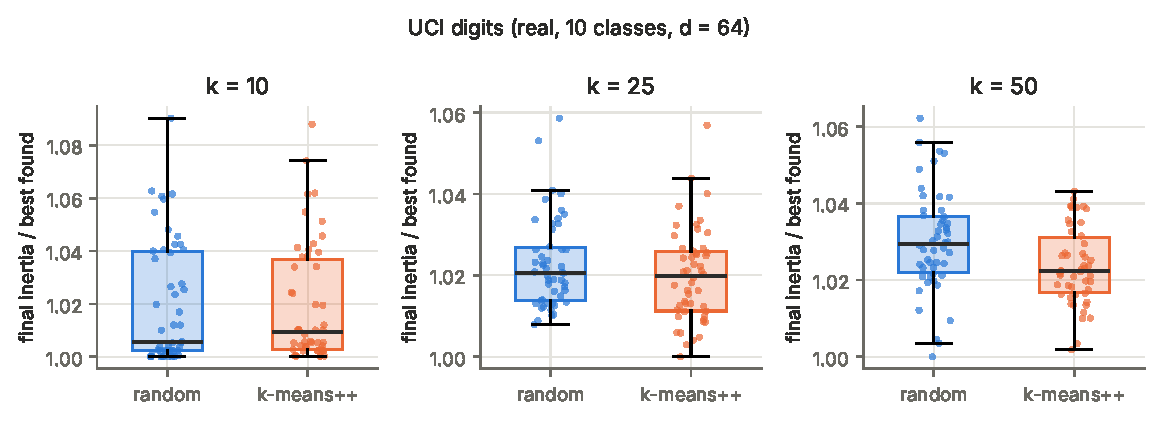
\includegraphics[width=\textwidth]{figures/digits_box.pdf}
\caption{UCI Digits: distribution of final inertia relative to the best found
(linear scale; note how narrow the range is compared with Figure~\ref{fig:normbox}).}
\label{fig:digbox}
\end{figure}

On Digits (Table~\ref{tab:Digits}, Figure~\ref{fig:digbox}) the picture is very
different: \textbf{all runs of both methods end within 9\% of the best}, and the
mean ratios are close (1.020 vs 1.019 for $k=10$; 1.023 vs 1.020 for $k=25$;
1.030 vs 1.024 for $k=50$). k-means++ has a slightly lower mean and, for larger
$k$, a lower worst case (ratio max 1.043 vs 1.062 at $k=50$) and lower CV
(0.97\% vs 1.27\%). Its seeding cost is lower in all cases, but only by a few
percent (seed ratio 1.93 vs 1.96 for $k=10$). The pair ARI is practically
identical ($\approx0.75$ for $k=10$), so the partitions found are as unstable
with either seeding, and the ARI with the true digit classes is $\approx0.61$ for
both: k-means captures much of the digit structure but cannot separate classes
such as 1, 7 and 9 that are not compact, well-separated blobs in pixel space.
Convergence speed is also similar (about 19--20 iterations, Figure~\ref{fig:conv},
right), and the seeding overhead of k-means++ is negligible at this scale (all
runs take tens of milliseconds).

Why so little difference? Real data in 64 dimensions does not consist of well
separated blobs: the classes overlap and the inertia landscape has many local
minima of very similar cost. Random points already fall in every dense region,
so there is little room for a clever seeding to help. This is consistent with the
paper, where the gains on real datasets are smaller than on Norm-25.
The held-out check confirms that the centres generalize: with $k=10$ the average
per-point cost is $658.3$ (train) vs $688.1$ (test) for random seeding and
$656.3$ vs $684.1$ for k-means++; the small train/test gap is the same for both
methods, so better seeding does not mean overfitting.

\subsection{Stability across seeds}

\begin{figure}[ht]\centering
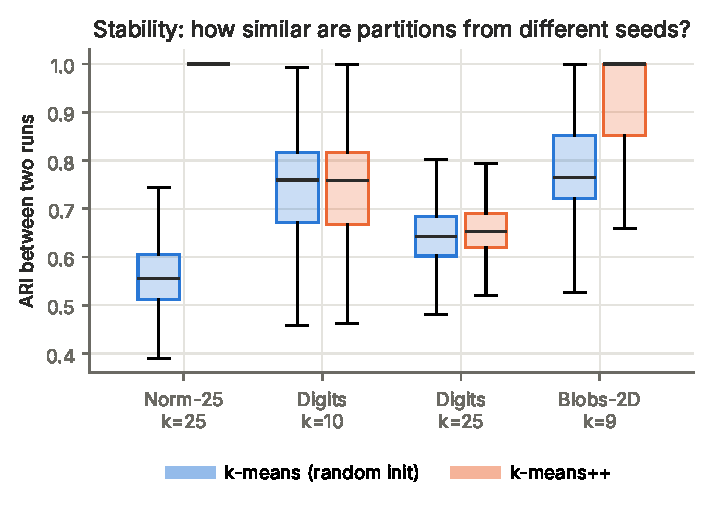
\includegraphics[width=0.68\textwidth]{figures/stability_pairwise_ari.pdf}
\caption{ARI between the partitions of every pair of runs (1225 pairs per box).}
\label{fig:stab}
\end{figure}

Figure~\ref{fig:stab} summarizes stability from the point of view of the
\emph{output}. When the data has a clear cluster structure that matches $k$
(Norm-25, Blobs-2D), k-means++ is far more stable: on Norm-25 it returns the very
same partition every time, while two random runs agree only at ARI $\approx0.56$.
On Digits both seedings are equally unstable, because the instability comes from
the data (many near-optimal partitions), not from the seeding.

\subsection{Extensions: overlapping clusters and dimensionality}

\begin{figure}[ht]\centering
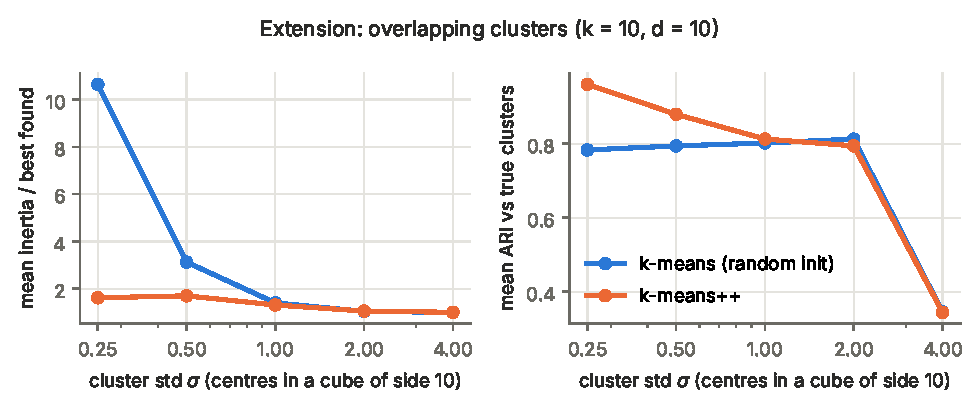
\includegraphics[width=\textwidth]{figures/ext_overlap.pdf}
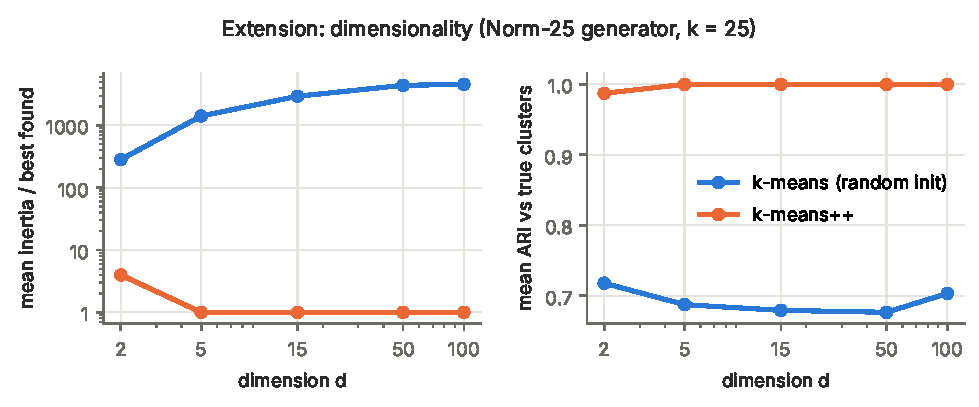
\includegraphics[width=\textwidth]{figures/ext_dimension.pdf}
\caption{Top: increasing cluster overlap. Bottom: increasing dimension. Means
over 20 paired runs per point.}
\label{fig:ext}
\end{figure}

\paragraph{Overlap.} With well-separated clusters ($\sigma=0.25$) random seeding
ends on average at 10.6 times the best cost against 1.6 for k-means++ (ARI with
truth 0.78 vs 0.96). As $\sigma$ grows the advantage shrinks, and from $\sigma=1$
on the two methods are indistinguishable; at $\sigma=4$ the clusters are mixed so
much that both recover the truth poorly (ARI $\approx0.34$) while the cost is
within 0.6\% of the best for both. In other words, the value of careful seeding is
largest exactly when there \emph{is} a clear structure to find, which is the same
conclusion as Norm-25 vs Digits. Note that k-means++ is not perfect even at
$\sigma=0.25$ (ratio 1.6), because with only 10 centres in a small cube some true
centres are close to each other.

\paragraph{Dimension.} With the Norm-25 generator, k-means++ is optimal in every
run for every $d\ge5$, while random seeding gets worse as $d$ grows (mean ratio
from about 280 at $d=2$ to about 4500 at $d=100$). The ARI of random seeding
stays around 0.7 for all $d$: the \emph{probability} of a bad seeding does not
depend on $d$ (it is the same ``balls into bins'' event), but the \emph{price} of
a merged pair of clusters grows linearly with $d$, since the squared distance
between two random points of the cube does. At $d=2$ some true centres happen to
be close, so k-means++ loses a little (ratio 4.0, ARI 0.99).

\section{Discussion and conclusions}

\paragraph{What we observed.}
\begin{enumerate}
\item Initialization can change the \emph{final} k-means cost by more than three
orders of magnitude on data with well separated clusters, and Lloyd's algorithm
cannot fix a bad start: it only moves centres locally.
\item k-means++ removes this failure mode almost completely: on Norm-25 it found
the best solution in 100\% of runs, in a single Lloyd iteration, and its seeding
cost is far below the theoretical bound $8(\ln k+2)$.
\item Its benefits are much smaller on real, overlapping data (Digits), where all
local minima have similar cost; there it is still never worse on average and has
a slightly better worst case.
\item The cost alone can hide instability: for $k=50$ on Norm-25 and on Digits,
runs with almost the same inertia return clearly different partitions.
\end{enumerate}

\paragraph{Limitations.} The ``best'' inertia is the best found, not a certified
optimum; 50 trials estimate the tails of the distribution only roughly; Digits is
one real dataset of moderate size, and we did not tune the number of clusters or
compare with other remedies (multiple restarts, which scikit-learn uses by
default, or greedy k-means++ that samples several candidates per step). Timing
comparisons at this scale are dominated by Python overhead and should not be read
as general conclusions. Finally, k-means++ does not fix the deeper limitations of
the k-means objective itself (spherical, equally sized clusters), which is visible
in the modest ARI on Digits.

\paragraph{Reproducibility.} \texttt{pip install -r requirements.txt}, then
\texttt{python run\_experiments.py} regenerates every figure, every table of this
report (\texttt{report/tables.tex}) and the raw results in \texttt{results/} in
under a minute; all randomness is controlled by explicit seeds.

\section*{References}
\begin{itemize}
\item D.\ Arthur and S.\ Vassilvitskii. \emph{k-means++: The Advantages of Careful
Seeding}. SODA 2007.
\item S.\ Lloyd. \emph{Least squares quantization in PCM}. IEEE Trans.\
Information Theory, 1982.
\item L.\ Hubert and P.\ Arabie. \emph{Comparing partitions}. Journal of
Classification, 1985.
\item E.\ Alpaydin and C.\ Kaynak. \emph{Optical Recognition of Handwritten Digits}.
UCI Machine Learning Repository, 1998.
\end{itemize}

\section*{Declaration}
I declare that this material, which I now submit for assessment, is entirely my
own work and has not been taken from the work of others, save and to the extent
that such work has been cited and acknowledged within the text of my work. I
understand that plagiarism, collusion, and copying are grave and serious offences
in the university and accept the penalties that would be imposed should I engage
in plagiarism, collusion or copying. This assignment, or any part of it, has not
been previously submitted by me or any other person for assessment on this or any
other course of study.

\end{document}
